One of the shortcomings of our hybrid system as described in
Chapters~\ref{chap:Hybrid_Cache} and~\ref{chap:Eviction_Strategies} is that it
only utilizes an individual node's RAM\@. When data is evicted, it moves
straight out of memory, either to be removed from the cache as a whole or
placed into S3. In EC2 an individual node's memory comprises a fairly small
fraction of its total storage. For example, the \emph{Extra Large instance}
type, {\tt m1.xlarge} consists of 15GB of memory and \emph{1,690GB} of disk
space.  RAM comprises less than 1\% of the overall storage capacity of the
instance.

In this chapter we create a cache that takes advantage of the extra storage
capacity, detail the necessary modifications to existing eviction strategies,
and present a Cost Aware data placement strategy. Further, we demonstrate
through experimental results that the Cost Aware strategy outperforms our
LRU-based eviction strategy.

\section{Storage Hierarchy} % (fold)
\label{sec:storage_hierarchy}
As mentioned, our previous cache configurations utilize only a small portion of
the total storage capacity of each individual instance. Recall from
Chapter~\ref{chap:Background} our main priority in our Elastic Key-Value Cache
system is to provide fast access to data. To support this, we utilized only
main memory. As a node's memory filled, we would then allocate further
instances to handle the overflow.

In Section~\ref{sub:aws_tradeoffs} we further discuss a number of trade-offs
between each storage medium. This has a side-effect of establishing a storage
hierarchy based on the performance of each medium.

\begin{figure}
\begin{center}
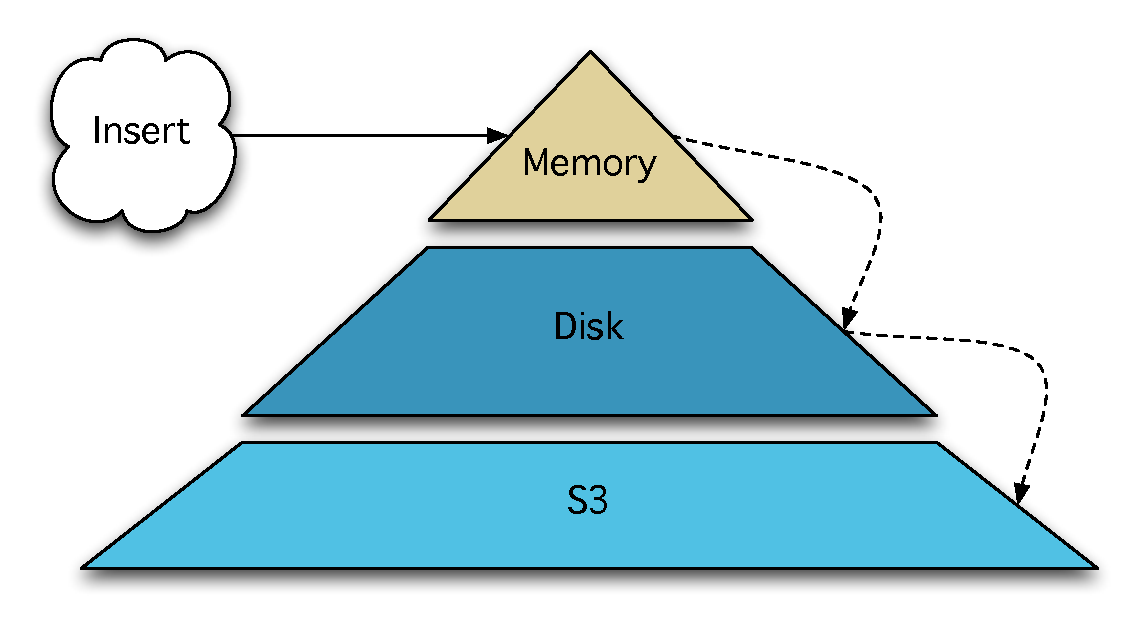
\includegraphics[scale=0.5]{figures/hierarchy-lru.pdf}
\end{center}
\caption{Hierarchy Structure for LRU}
\label{fig:hierarchy_lru}
\end{figure}

\subsection{Memory} % (fold)
\label{sub:storage_memory}
Because the data here exists in the core of the instance, memory offers the
highest performance of the three storage mediums. However, as mentioned,
storage space is at a premium. Table~\ref{tab:mem_ec2_instance} outlines the
storage capacities of the standard instance sizes. In each case, memory
comprises approximately 1\% or less of the overall storage capacity of an
individual instance. For this reason, we argue that memory should compose the
highest level of the hierarchy.

\begin{table}[htp]
  \begin{center}
    \begin{tabular}{|c|c c| c|}
      \hline
      \multicolumn{1}{|c}{\textbf{Instance Type}} &
      \multicolumn{1}{|c}{\textbf{Memory}} &
			\multicolumn{1}{c|}{\textbf{Disk}} &
			\multicolumn{1}{c|}{\textbf{Percentage of total}}\\
      \hline
			Small (Default)     & 1.70GB & 160GB & 1.05\%\\
								   Medium & 3.75GB & 410GB & 0.91\%\\
						        Large & 7.50GB & 850GB & 0.87\%\\
				      Extra Large & 15.0GB & 1,690GB & 0.88\%\\
      \hline
    \end{tabular}
    \caption{EC2 Instance Storage Capacity}
    \label{tab:mem_ec2_instance}
  \end{center}
\end{table}

% subsection storage_memory (end)

\subsection{Disk} % (fold)
\label{sub:storage_disk}
Though the disk offers 100-fold increases in storage capacity, this extra space
comes at a cost. Compared to memory accesses, disk accesses can be very slow.
It is possible, however, that if the average data size is large, disk access
overheads may be amortized over time. For this reason, the instance's disk acts
as the second level of our three-tier storage hierarchy.

% subsection storage_disk (end)

\subsection{Cloud} % (fold)
\label{sub:storage_cloud}
The final layer of our hierarchy consists of our persistent, cloud-based
storage option. For our purposes, we consider Amazon's S3 service once again.
S3 provides us with a monumental amount of storage space (effectively
``infinite''), persistence in the event of node failure or contraction, and a
secondary region to which service demands can be redirected. However, due to
the reliability and availability guarantees Amazon makes for S3, the storage
architecture is implemented in such a robust fashion that performance is
impacted. For this reason, S3 acts as the final, but largest layer of our
storage hierarchy.

We do not consider the effects of using the Elastic Block Storage (EBS) volumes
for this purpose. Purely as conjecture, because these EBS volumes are mounted
to the instance, we expect the performance of such a layer to closely mimic
that of the disk. Further, as EBS volume sizes must be predefined, the primary
benefit of such a layer would be its persistence and the ability to supplement
the existing disk layers of already-running instances, losing the size and
flexibility benefits of S3.
% subsection storage_cloud (end)

% section storage_hierarchy (end)

\section{Metadata and the Rolodex} % (fold)
\label{sec:rolodex}
This new hierarchy creates certain challenges with the management of our data.
We can no longer assume that data is stored in memory, and, in the event of
search failure, default to checking our cloud. Though we could perform a three
step search, traveling down our storage hierarchy as each previous layer
results in a miss, this is prohibitive. For this reason we associate metadata
with each key-value pair.

\begin{table}[htp]
  \begin{center}
    \begin{tabular}{|c|l|}
      \hline
      \multicolumn{1}{|c}{\textbf{Metadata}} &
      \multicolumn{1}{|c|}{\textbf{Description}}\\
      \hline
					Hits & Number of times this element has been accessed\\
					Size & Size (in bytes) of this element's data\\
		  Location & Which layer the data is stored in (used for retrieval)\\
Retrieval Time & The amount of time this data took to retrieve from the
			secondary data source\\
	 Last Access & The time at which the data was last accessed\\
		Last Reset & The time at which the hit count was last reset\\
	Last Scoring & The time at which this index was last scored\\
				 Score & The score for this index\\
      \hline
    \end{tabular}
    \caption{Index Metadata}
    \label{tab:metadata}
  \end{center}
\end{table}

Table~\ref{tab:metadata} displays the various pieces of information we maintain
for each key-value pair. Many of these elements are unnecessary for the
purposes of data retrieval and a LRU-based eviction scheme. In fact, in this
case, only the size, location, and last-access data members serve any purpose.
We maintain the remaining metadata however, as it will come into play when we
introduce our Cost Aware scoring algorithm later in the chapter. This metadata
is then stored in a structure we call the \emph{Rolodex}.

The Rolodex operates much like its namesake, where each index card is
associated with a certain key-value pair (indexed on the unique key) and
contains the associated metadata. While technically this only describes a hash
table--and in fact, that is how the indices are stored--this structure offers
additional functionality for maintaining and interacting with the data, such as
the ability to retrieve all elements stored in certain locations, all elements
with access times past certain time stamps, the ability to compute access
frequencies, and apply scoring algorithms to each index. As elements are
accessed in the Rolodex, it also updates the requisite information stored in
the metadata such as hit count and last-access timestamps.

The existence of this Rolodex allows us to more efficiently perform searches as
demonstrated in Algorithm~\ref{alg:hierarchy_search}. We need only perform a
retrieval of the metadata associated with a key to discover the storage
location of our data. If no such data exists, we can simply return NULL\@.
Because our Rolodex is essentially a wrapper to a hash table, these lookups are
performed in $O(1)$ time.

As a note, the three identifiers {\tt :memory}, {\tt :disk} and {\tt :cloud}
are all arbitrarily defined symbols. This syntax is borrowed from Ruby where a
colon preceding a word indicates that the word is a ``symbol''. In essence,
they are named identifiers for the locations in which the data is placed. This
could be performed equally as well with integers, \eg 1, 2 and 3 for memory,
disk and cloud respectively.

\begin{algorithm}[htp]
\small
\caption{\label{alg:hierarchy_search}hierarchy\_search($key$)}
\begin{algorithmic}[1]
\STATE $meta \leftarrow rolodex$.search($key$)

\IF{$meta =$ NULL}
  \STATE return NULL
\ENDIF

\STATE $rolodex$.update($key$)

\IF{$meta$.location $=$ {\tt :memory}}
	\STATE $memory\_queue$.update($key$)
	\STATE \textbf{return} $memory$.search($key$)
\ELSIF{$meta$.location $=$ {\tt :disk}}
	\STATE $disk\_queue$.update($key$)
	\STATE \textbf{return} $disk$.search($key$)
\ELSIF{$meta$.location $=$ {\tt :cloud}}
	\STATE $cloud\_queue$.update($key$)
	\STATE \textbf{return} $cloud$.search($key$)
\ENDIF
\end{algorithmic}
\end{algorithm}

% section rolodex (end)

\section{LRU-Based Insertion and Eviction} % (fold)
\label{sec:storage_insertion_eviction}
By establishing this hierarchy of storage mediums, we naturally necessitate
changes to the insertion and eviction algorithms of the cache. In keeping with
the results of the previous chapter, we continue to use LRU priority queues to
manage our cache eviction. Figure~\ref{fig:hierarchy_lru} outlines the general
structure of our LRU-based system, while Algorithms~\ref{alg:insert_lru}
through~\ref{alg:evict_disk_lru} demonstrate them in further detail.

\begin{algorithm}[htp]
\small
\caption{\label{alg:insert_lru}insert\_lru($key$, $value$, $retrieval\_time$)}
\begin{algorithmic}[1]
\STATE $\triangleright$ Obtain the global eviction queue $memory\_queue$
\STATE $size \leftarrow value$.size

\IF{!$memory$.fits($size$)}
  \STATE evict\_from\_memory($size$)
\ENDIF

\STATE $memory$.insert($key$, $value$)
\STATE $memory\_queue$.add($key$)
\STATE $rolodex$.add($key$, $size$, $retrieval\_time$, {\tt :memory})
\end{algorithmic}
\end{algorithm}

\begin{algorithm}[htp]
\small
\caption{\label{alg:evict_mem_lru}evict\_from\_memory($size$)}
\begin{algorithmic}[1]
\STATE $\triangleright$ Obtain the global eviction queues $memory\_queue$ and
$disk\_queue$, $threshold$, and $disk$ broker
\STATE $memory\_limit \leftarrow memory$.size $* threshold$

\STATE $\triangleright$ Continue evicting until our memory is beneath our
threshold and we can fit the new element in
\WHILE{$(memory\_limit > memory$.size$)$ and \@!$memory$.fits($size$)}
  \STATE $\triangleright$ obtain the evicted key from our eviction queue
  \STATE $key \leftarrow memory\_queue$.shift
  \STATE $value \leftarrow memory$.search($key$)

	\STATE $evict\_size \leftarrow rolodex$.search($key$).size

	\IF{!$disk$.fits($evict\_size$)}
		\STATE evict\_from\_disk($evict\_size$)
	\ENDIF

  \STATE $memory$.delete($key$)
  \STATE $disk$.insert($key$, $value$)
	\STATE $disk\_queue$.push($key$)
	\STATE $rolodex$.search($key$).location $\leftarrow$ {\tt :disk}
\ENDWHILE
\end{algorithmic}
\end{algorithm}

\begin{algorithm}[htp]
\small
\caption{\label{alg:evict_disk_lru}evict\_from\_disk($size$)}
\begin{algorithmic}[1]
\STATE $\triangleright$ Obtain the global eviction queues $disk\_queue$ and
$cloud\_queue$, $threshold$, and $cloud$ broker
\STATE $disk\_limit \leftarrow disk$.size $* threshold$

\STATE $\triangleright$ Continue evicting until our disk is beneath our
threshold and we can fit the new element in
\WHILE{$(disk\_limit > disk$.size$)$ and \@!$disk$.fits($size$)}
  \STATE $\triangleright$ obtain the evicted key from our eviction queue
  \STATE $key \leftarrow disk\_queue$.shift
  \STATE $value \leftarrow disk$.search($key$)
  \STATE $disk$.delete($key$)
  \STATE $cloud$.insert($key$, $value$)
	\STATE $cloud\_queue$.push($key$)
	\STATE $rolodex$.search($key$).location $\leftarrow$ {\tt :cloud}
\ENDWHILE
\end{algorithmic}
\end{algorithm}

In this way, data is initially inserted into memory. Only once memory has
become full do we begin to evict, moving data from memory to disk. Similarly,
once the disk has become full, we cascade into
Algorithm~\ref{alg:evict_disk_lru} and move data from the disk to S3. Performed
this way, the cache will always try to take advantage of the higher tiers in the
hierarchy, only resorting to the final tier when the other two have filled.

In many ways this is very similar to the algorithms defined in
Chapter~\ref{chap:Hybrid_Cache}. The primary difference is that of the Rolodex
and the secondary tier of eviction (memory to disk, and disk to S3 rather than
memory to S3).
% section storage_eviction (end)

\section{Cost Aware Data Placement} % (fold)
\label{sec:cost-aware}
In this section, we introduce the concept of a Cost Aware data placement
algorithm. One of the perceived weaknesses of the LRU-based eviction system is
that it does not efficiently make use of the resources provided. Data is placed
into one of the three mediums based entirely on its time since last usage,
however this can easily result in memory being monopolized by only a small set
of values. If the request frequency is low, these values will clear out
eventually, moving onto disk. However we argue that it is better for memory to
consist of a large set of smaller files rather than a small set of larger
files, given similar access frequencies.

For this purpose we need a scoring algorithm that takes a number of key
elements into account, access frequency, retrieval time, and size foremost
amongst them. The specifics of our scoring algorithm will be introduced later,
at the moment, we will explore the changes to our insertion algorithm and the
updated data placement algorithm.

\begin{algorithm}[htp]
\small
\caption{\label{alg:insert_ca}insert\_ca($key$, $value$, $retrieval\_time$)}
\begin{algorithmic}[1]
\STATE $size \leftarrow value$.size
\STATE $location \leftarrow$ {\tt :cloud}

\IF{$memory$.fits($size$)}
  \STATE $memory$.insert($key$, $value$)
	\STATE $location \leftarrow$ {\tt :memory}
\ELSIF{$disk$.fits($size$)}
	\STATE $disk$.insert($key$, $value$)
	\STATE $location \leftarrow$ {\tt :disk}
\ELSE
	\STATE $cloud$.insert($key$, $value$)
\ENDIF

\STATE $rolodex$.add($key$, $size$, $retrieval\_time$, $location$)
\end{algorithmic}
\end{algorithm}

Algorithm~\ref{alg:insert_ca} is actually much simpler than that of the
previous, LRU-based eviction scheme. Data is simply placed into the first
medium that has space. The data placement algorithm is performed in a
background thread and executes continually over the duration of the cache's
existence.  This algorithm is described in
Algorithm~\ref{alg:ca_data_placement}.

\begin{algorithm}[htp]
\small
\caption{\label{alg:ca_data_placement}ca\_data\_placement()}
\begin{algorithmic}[1]
\WHILE{$\triangleright$ server is running}
	\STATE update\_metas()

	\STATE $new\_size\_mem \leftarrow 0$
	\STATE $new\_size\_disk \leftarrow 0$
	\STATE $memory\_candidates \leftarrow$ Array.new
	\STATE $disk\_candidates \leftarrow$ Array.new
	\STATE $cloud\_candidates \leftarrow$ Array.new

	\STATE $\triangleright$ sort the Rolodex into descending order by scores and
	iterate over each (key,meta) pair finding where they belong
	\FORALL{$(key, meta) \in rolodex$.sort\_by\_score}
		\STATE $\triangleright$ if this candidate fits into memory and it is not
		already there, we place it as a candidate
		\IF{$new\_size\_mem + meta$.size $< memory$.max\_size}
			\IF{$meta$.location $\neq$ {\tt :memory}}
				\STATE $memory\_candidates$.push($key$)
			\ENDIF
			\STATE $new\_size\_mem += meta$.size
		\ELSIF{$new\_size\_disk + meta$.size $< disk$.max\_size}
			\IF{$meta$.location $\neq$ {\tt :disk}}
				\STATE $disk\_candidates$.push($key$)
			\ENDIF
			\STATE $new\_size\_disk += meta$.size
		\ELSE
			\IF{$meta$.location $\neq$ {\tt :cloud}}
				\STATE $cloud\_candidates$.push($key$)
			\ENDIF
		\ENDIF
	\ENDFOR

	\FORALL{$key \in cloud\_candidates$}
		\STATE $meta \leftarrow rolodex$.search($key$)
		\STATE $\triangleright$ migrate from $meta$.location to {\tt :cloud}
		\STATE $meta$.location $\leftarrow$ {\tt :cloud}
	\ENDFOR
	
	\FORALL{$key \in disk\_candidates$}
		\STATE $meta \leftarrow rolodex$.search($key$)
		\STATE $\triangleright$ migrate from $meta$.location to {\tt :disk}
		\STATE $meta$.location $\leftarrow$ {\tt :disk}
	\ENDFOR

	\FORALL{$key \in memory\_candidates$}
		\STATE $meta \leftarrow rolodex$.search($key$)
		\STATE $\triangleright$ migrate from $meta$.location to {\tt :memory}
		\STATE $meta$.location $\leftarrow$ {\tt :memory}
	\ENDFOR
\ENDWHILE
\end{algorithmic}
\end{algorithm}

\begin{algorithm}[htp]
	\small
	\caption{\label{alg:ca_update_metas}update\_metas()}
	\begin{algorithmic}[1]
	\STATE $current\_time \leftarrow$ Time.now
	\STATE $\triangleright$ rescore all values in the Rolodex where the time
	since the last scoring is over some threshold $T_{score}$
	\FORALL{$meta \in rolodex$}
		\IF{$current\_time - meta$.last\_scoring $> T_{score}$}
			\STATE $meta$.rescore
			\STATE $meta$.last\_scoring $\leftarrow current\_time$
		\ENDIF
	\ENDFOR
	
	\STATE $\triangleright$ reset all values in the Rolodex where the time
	since the last reset is over some threshold $T_{reset}$
	\FORALL{$meta \in rolodex$}
		\IF{$current\_time - meta$.last\_reset $> T_{reset}$}
			\STATE $meta$.hits $\leftarrow 0$
			\STATE $meta$.last\_reset $\leftarrow current\_time$
		\ENDIF
	\ENDFOR
\end{algorithmic}
\end{algorithm}

Algorithm~\ref{alg:ca_data_placement} begins by executing
Algorithm~\ref{alg:ca_update_metas}. This algorithm simply updates the scores
of meta data that has not recently been re-scored. Parameters $T_{score}$ and
$T_{reset}$ are experimental parameters that control the amount of time between
re-scoring and resetting the hit count respectively. $T_{score}$ is important for
maintaining smooth operation, as it directly controls the number indices
that are being re-scored and indirectly, the potential number of data elements
that must later be migrated. $T_{reset}$, on the other hand, is important for
ensuring the freshness of trends. While the scoring algorithm is certainly
capable of assessing penalties over time, resetting the hit count of indices
prevents large trends from dominating the access history by limiting frequency
assessments to certain time windows.

Following this, the Rolodex is sorted into descending order by score. Data is
then organized into candidate locations based on the hierarchy. The placement
of these elements operate in a cascading manner. Initially, the algorithm
attempts to place the element into memory, succeeding only if it fits. If
successful and the element is not already contained in memory, the key is
placed into the $memory\_candidates$ queue. Even if the element is already in
memory, we increment the $new\_size\_mem$ value with the size of the data to
acknowledge the fact that this element will be stored within. If the data
cannot be placed into memory, the same process is duplicated with the disk.
Failing that, data is placed onto the cloud. By cascading in this manner, data
with a higher score may still be placed into memory over one with a lower score
simply because it fits. This process ensures that each layer is filled more
fully than if a ``does not fit'' response triggered all subsequent elements
being placed in the following storage tier.

Finally, data is migrated from its current location to its candidate location.
This is done in reverse order, first moving elements into the cloud so as to
evacuate the contents of memory and disk. This is important, as in
space-limited environments, moving to memory or disk first could overflow their
max contents. Data is then moved to disk so that things are properly removed
from memory beforehand. And, at last, data is moved into memory.

\subsection{Scoring} % (fold)
\label{sub:ca_scoring}
Throughout this section, we have left the scoring algorithm something of a
mystery. This is to demonstrate that the cost aware cache operates somewhat
agnostic to the scoring mechanism. The only expectation made in
Algorithm~\ref{alg:ca_data_placement} is that the most important elements have
larger scores than others. However, even this can be changed simply by
modifying the direction of the sort on the Rolodex at line 9.

For our purposes, we developed an algorithm taking heavy influence from TF-IDF
and Okapi BM25\cite{tfidf,bm25}, two widespread ranking algorithms in
information retrieval. In addition to the access frequency of data elements, we
consider their size relative to storage mediums, the amount of time these
elements took to retrieve from the original source, and a time factor. Scoring
is described in Equation~\ref{eqn:scoring} through~\ref{eqn:time} and the
variables being used are outlined in Table~\ref{tab:scoring_variables}.

\begin{table}[htp]
  \begin{center}
    \begin{tabular}{|c|l|}
      \hline
      \multicolumn{1}{|c}{\textbf{Variable}} &
      \multicolumn{1}{|c|}{\textbf{Description}}\\
      \hline
				$D$ & Data object\\
				$|D|$ & Data size\\
				$D_t$ & Data's last access time\\
				$D_h$ & Number of hits on data object\\
				$r$ & Total number of requests to the cache\\
				$N$ & Storage node\\
				$N_R$ & Size of RAM in node\\
				$f(D)$ & Access frequency of the data object\\
				$c(D)$ & Retrieval cost\\
				$t(d)$ & Time factor\\
				$T_{now}$ & Current time\\
				$\beta,\alpha,\epsilon$ & User-defined tuning parameters\\
      \hline
    \end{tabular}
    \caption{Scoring algorithm variables}
    \label{tab:scoring_variables}
  \end{center}
\end{table}

\begin{equation}
	S(D) = \beta \left(1 - \frac{|D|}{N_R}\right) + (1 - \beta) * f(D) +
	\alpha*c(D) + \epsilon * t(D)
\label{eqn:scoring}
\end{equation}

\begin{equation}
	f(D) = \frac{D_h}{r}
\label{eqn:frequency}
\end{equation}

\begin{equation}
	t(D) = 1 - (T_{now} - D_t)
\label{eqn:time}
\end{equation}

The scoring equation is broken up into four different parts: \emph{size},
\emph{frequency}, \emph{retrieval}, and \emph{time}. By comparing the size as a
fraction of the total size of memory, those values which are equally as large
or larger result in much larger fractions. This is subtracted from 1 so that
values of $|D|$ closer to zero result in larger scores.

Frequency is then computed as the fraction of all requests which were devoted
to this data element. In this way, the more frequently accessed values are
given greater importance over those that have not been accessed many times.

The retrieval cost of a certain data element is further taken into account for
determining our overall importance. This part of the equation is most important in
caches supporting a service. As mentioned in the experimental section
Chapter~\ref{chap:Eviction_Strategies}, cache misses are associated with heavy
penalties. This is due to the way in which our elastic cache operates.
Figure~\ref{fig:architecture}, replicated here in
Figure~\ref{fig:architecture2} shows that a cache miss means that the
coordinator must execute a service. While this service may be as simple as
retrieving the data from another website, often these services can result in
the execution of very heavy computations. For this reason, we include the
retrieval cost of a value in our scoring considerations, insisting that those
values which take longer to compute are more important than those that do not.

\begin{figure}
\begin{center}
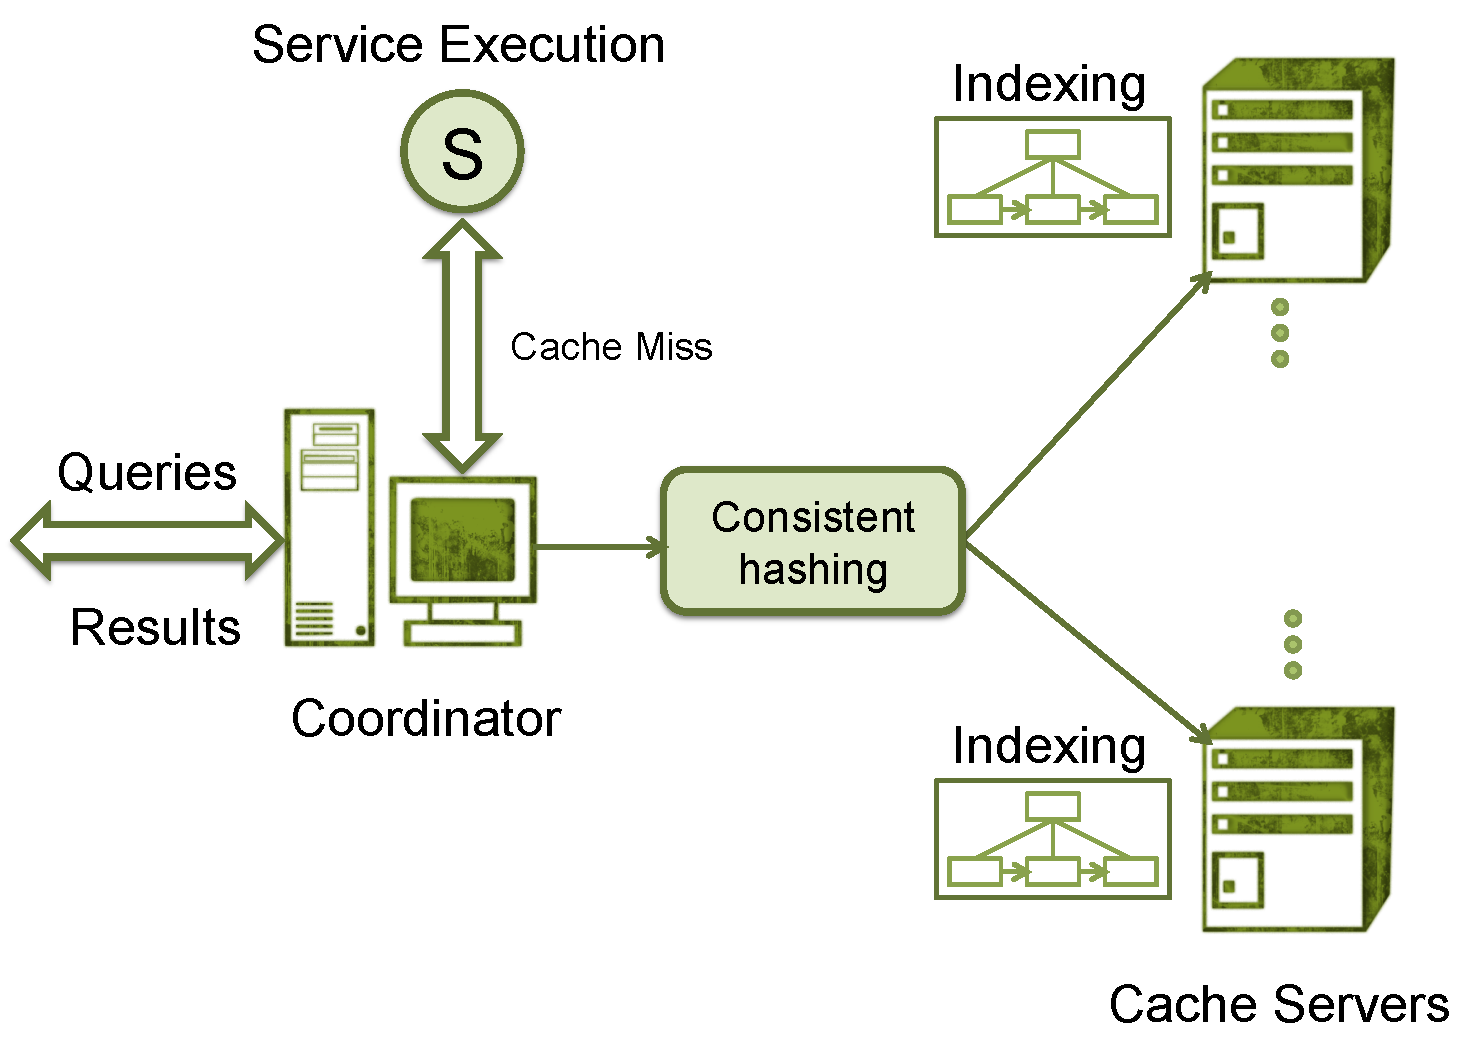
\includegraphics[scale=0.5]{figures/arch.pdf}
\end{center}
\caption{Client-Server Architecture of the Elastic Cache}
\label{fig:architecture2}
\end{figure}

Finally, we include as a consideration, the amount of time since the data was
last accessed. $t(D)$ operates similarly to the size portion of the equation.
Values of $D_t$ closer to the time at which the data is being rescored are
considered to be more important than those which have been accessed well into
the past.

The values $\alpha$, $\beta$, and $\epsilon$ are user-defined parameters that
control the weighting with which each portion of the equation is considered.
$\alpha$ controls the weighting of the retrieval time and $\epsilon$ controls
the importance of the time factor. $\beta$ serves a dual role, acting as a
balancing weight between the size and the frequency. A value of $0.5$ for
$\beta$ means that the two portions are considered equally, while values $<
0.5$ weigh more heavily towards the frequency and values $> 0.5$ weigh more
heavily towards the size factor.

% subsection ca_scoring (end)

% section cost-aware (end)

\section{Experiments} % (fold)
\label{sec:experiments_storage}
In these experiments we utilized four \emph{Large EC2 instances} ({\tt
m1.large}) from the Amazon Cloud each consisting of 7.5 GB of memory, 4 virtual
EC2 cores -- equivalent to a 1.0-1.2 GHz 2007 Opteron or 2007 Xeon Processor
each -- on 64 bit platforms.  Each instance was loaded with an Ubuntu Linux
image. These four instances are spread into two different regions, {\tt
us-east-1} (Virginia) and {\tt us-west-2}
(Oregon)\cite{amazonEC2locations}. In {\tt us-east-1} we host the
\emph{cache coordinator} and its single \emph{cache server}, as well as our
\emph{workload generator}. The instance in {\tt us-east-2} is a web server
hosting our \emph{data repository}. Figure~\ref{fig:ca-experiment-config}
contains a simple overview of the configuration.

\begin{figure}
\begin{center}
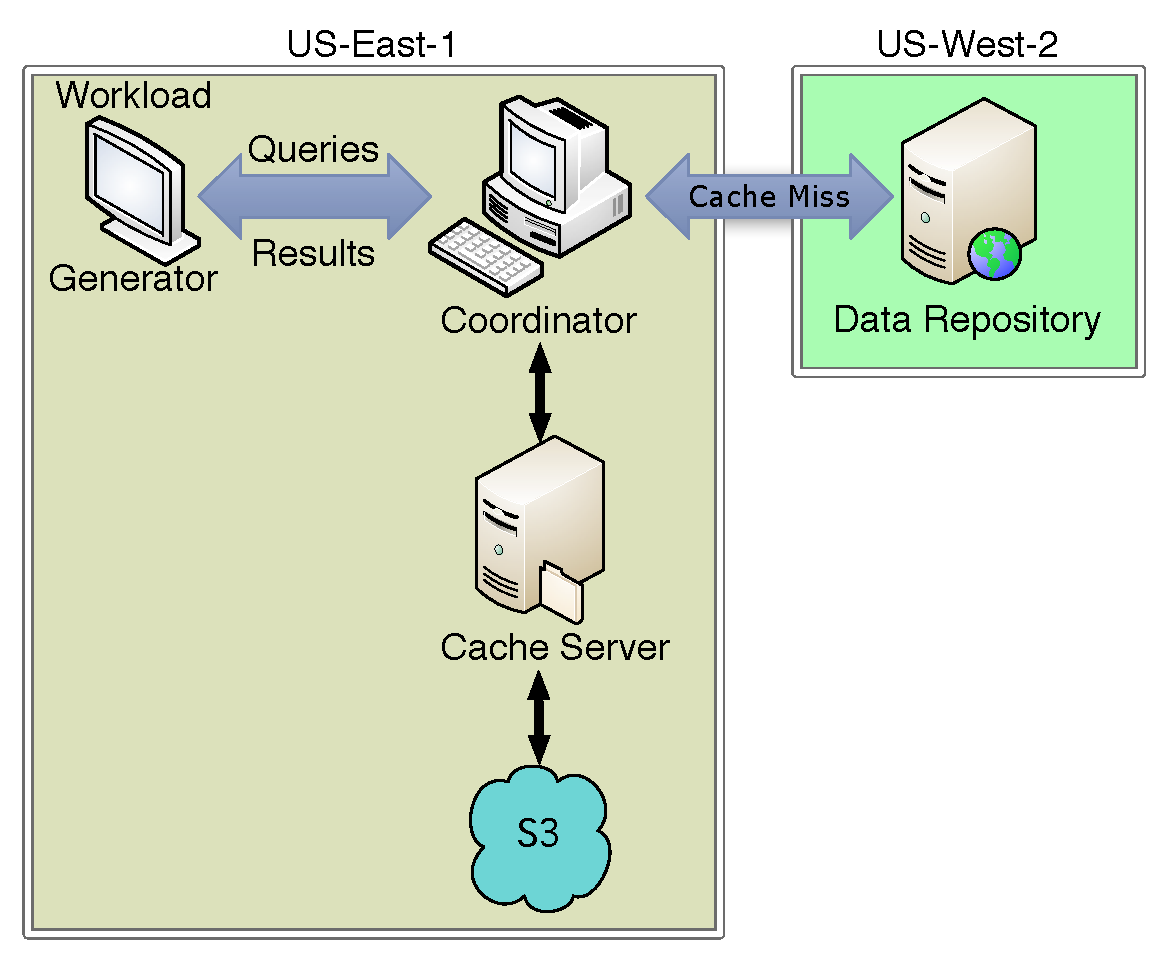
\includegraphics[scale=0.5]{figures/hierarchy-experiment-config.pdf}
\end{center}
\caption{Experimental Configuration}
\label{fig:ca-experiment-config}
\end{figure}

\subsection{Workload Generator} % (fold)
\label{sub:work_generator}
To evaluate the performance of our new hierarchical caching strategies we
created a \emph{workload generator} to simulate web traffic. This generator was
installed and run from an instance in the same AWS region as the cache ({\tt
us-east-1}). The generator is configured with the port number and hostname of
the cache coordinator as well as a file describing the traffic characteristics.
Once launched, it begins sending a stream of {\tt HTTP GET} requests to the
coordinator. All told, the generator executes 196,177 requests over a set of
15,000 unique keys.

Initially, this portion of the experimental configuration was meant to be
handled by a well-known, open source traffic generator called SURGE (Scalable
URL Reference Generator) from Boston University\cite{surge}. This tool offered
a number of features useful for generating representative web workloads,
amongst which were: file size distributions for the web server, Zipfian request
distributions, file popularity and individual client usage patterns including
idle periods. Sadly we encountered a number of problems with the tool, for
which the latest revision occurred in 1998. After spending significant amounts
of time attempting to debug SURGE ourselves, we resorted to developing our own
solution.

While our current traffic generator takes some cues from SURGE it is not as
fully featured. Most specifically, our traffic generator does not simulate the
individual client usage patterns and idle times are fairly static between
requests. It does however use the same data that SURGE generates for file size
distributions, request distributions and file popularity. In these experiments,
idle time is kept to a minimum, allowing each simulated client to proceed with
the next {\tt HTTP GET} request as soon as it has received and logged the
last.

% subsection work_generator (end)

\subsection{Data Repository} % (fold)
\label{sub:data_repository}
In past experiments our elastic cache has been used to support scientific
applications for which requested data must be generated through the execution
of some service. Once again, a reference to Figure~\ref{fig:architecture2}
demonstrates this configuration. In these situations, we have simulated this
service execution, which we presume to be quite costly due to the required
computations or the acquisition of the necessary data, by levying a 75 second
penalty for each cache miss. In this experiment we utilize our elastic cache to
support \emph{web service applications}.

Accordingly, our \emph{data repository} is configured with a back-end database
containing the data for our experiment (data which was generated by SURGE).
This web application acts as a key-value store where the key is the unique
filename and the value contains the contents of the file. This server is
installed and run on another EC2 instance located in a region separate from our
\emph{cache coordinator} ({\tt us-west-2} as opposed to {\tt us-east-1}). The
intent behind these separate locations is to introduce a slight degree of
network latency between the \emph{cache coordinator} and the \emph{data
repository}. This is representative of a very common scenario for web
applications.

\begin{figure}
\begin{center}
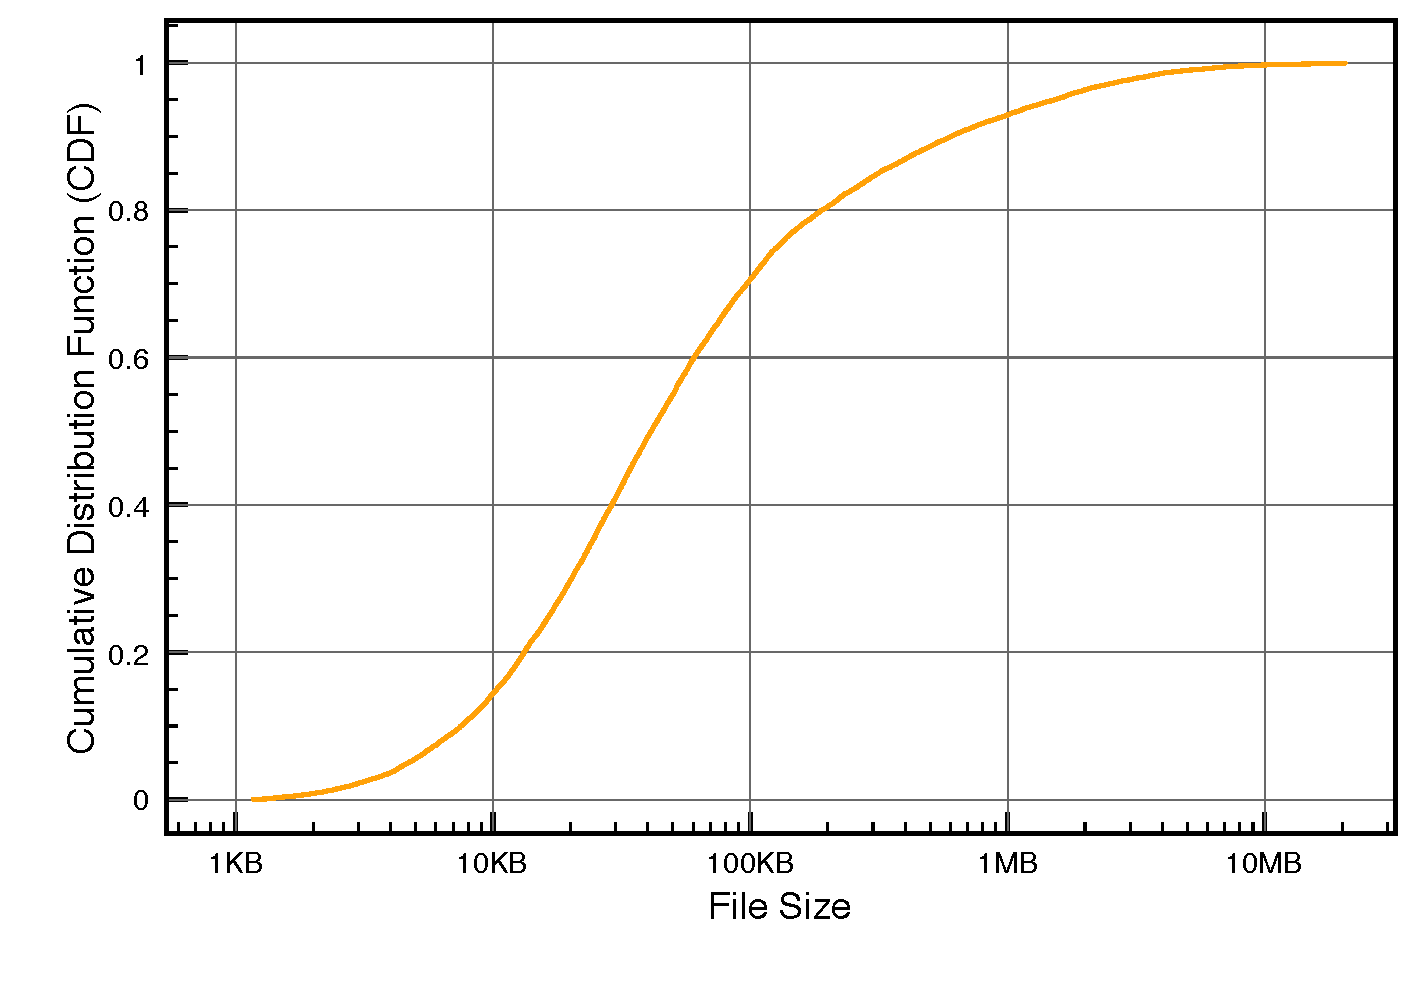
\includegraphics[scale=0.5]{figures/hierarchy-data-cdf.pdf}
\end{center}
\caption{CDF of file sizes on the web server}
\label{fig:file-cdf}
\end{figure}

Figure~\ref{fig:file-cdf} shows the \emph{Cumulative Distribution Function}
(CDF) of file sizes for the 15,000 files generated by SURGE for our \emph{data
repository}. The CDF displays the fraction of files in the data set that lie
within a specific range. Mathematically, given some value $X$, $CDF_x(X) = P(X
\leq x)$. Accordingly, the data files on our server range from 1KB to 10MB, and
approximately 75\% of those files are under 100KB in size. All told, the files
add up to roughly 4.2GB of data.

\begin{figure}
\begin{center}
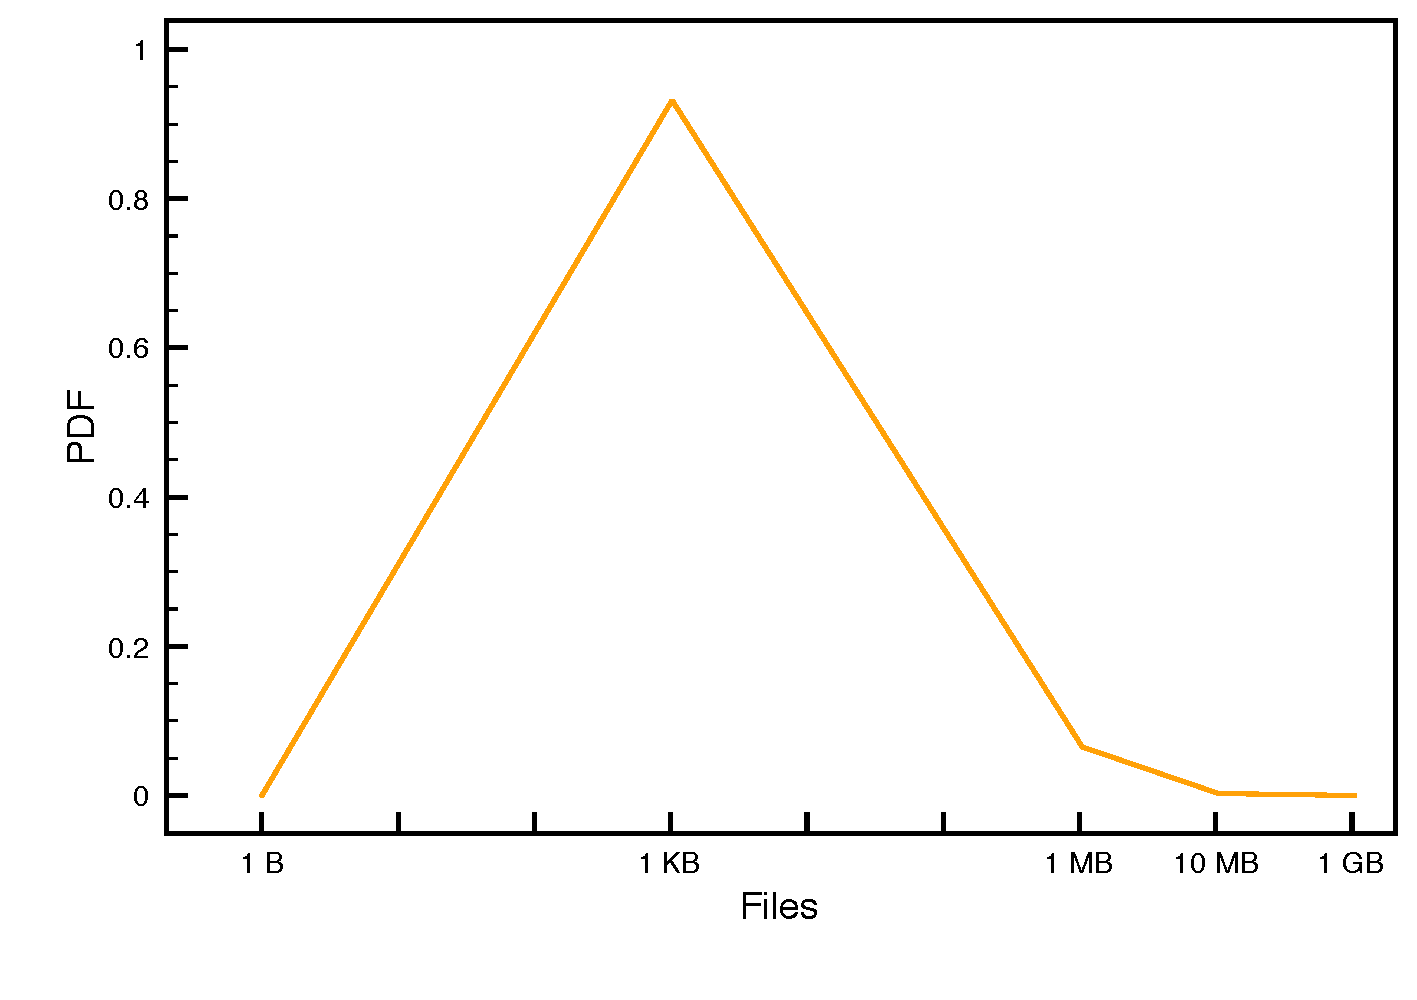
\includegraphics[scale=0.5]{figures/hierarchy-data-pdf-existence.pdf}
\end{center}
\caption{PDF of the likelihood that a file exists for a certain magnitude}
\label{fig:file-pdf-exists}
\end{figure}


\begin{figure}
\begin{center}
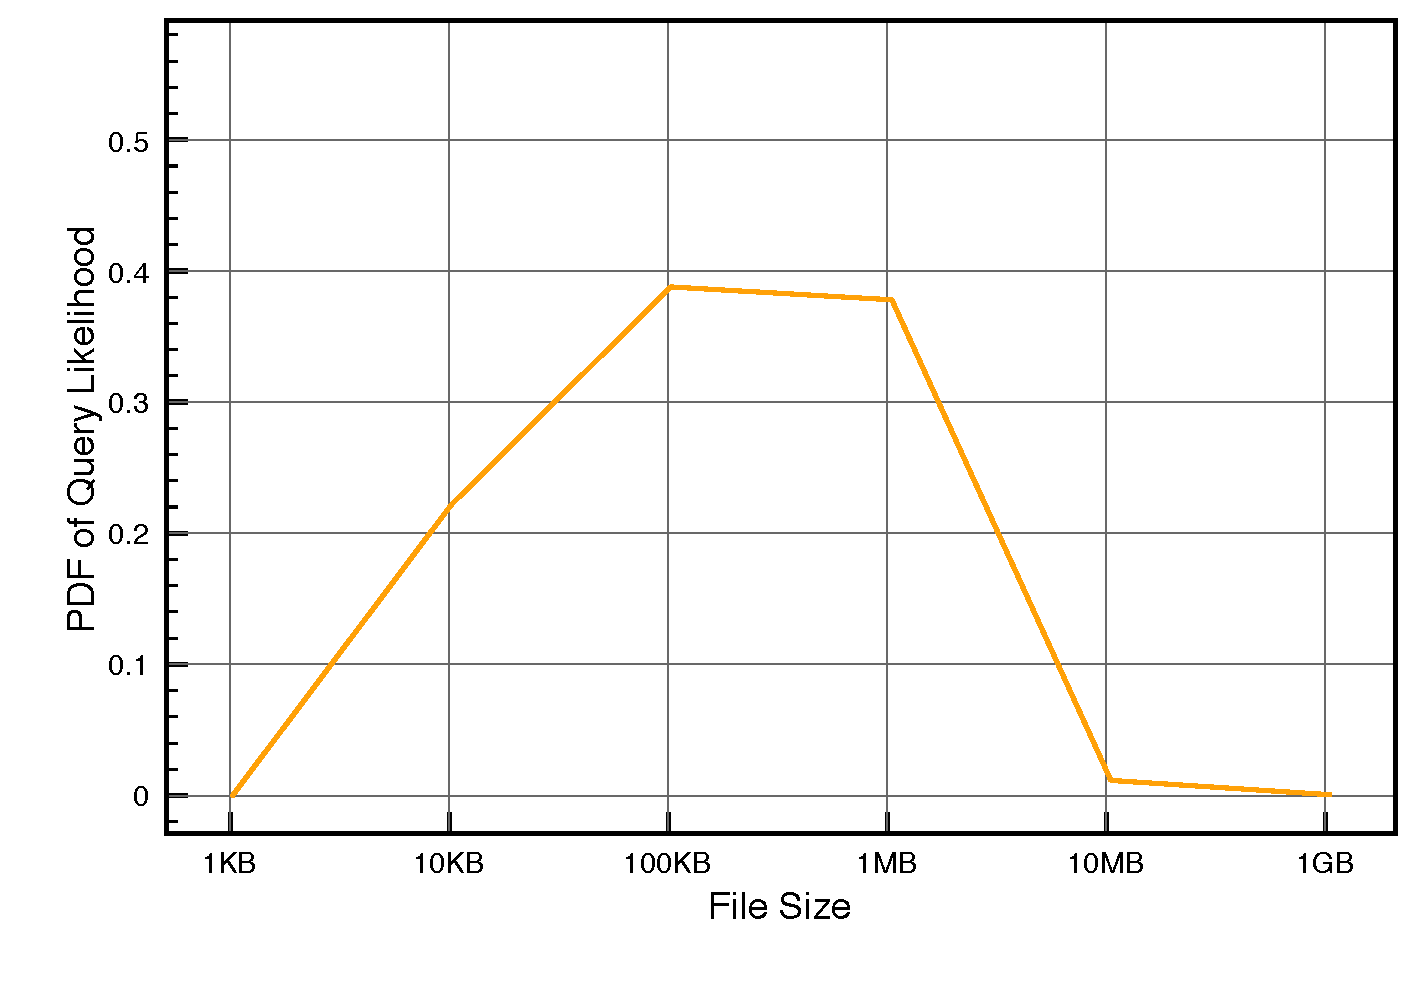
\includegraphics[scale=0.5]{figures/hierarchy-data-pdf-requests.pdf}
\end{center}
\caption{PDF of the likelihood that a query is for a file of a certain
magnitude}
\label{fig:file-pdf-requests}
\end{figure}

Figure~\ref{fig:file-pdf-exists} represents the \emph{Probability Density
Function} (PDF) for file size. That is, the likelihood that any given file in
our data set falls within a certain magnitude. Note that by this graph, 50\% of
our files fall between 10 and 100KB\@. Figure~\ref{fig:file-pdf-requests} shows
the PDF of \emph{query} likelihood,\ie the likelihood that any given request is
for a file of a certain magnitude. This demonstrates the query behavior of our
traffic generator, as the majority of requested files fall between 10KB and
1MB.
% subsection data_repository (end)

\subsection{Cache Configuration} % (fold)
\label{sub:cache_configuration}
The \emph{cache coordinator} is deployed on EC2 in the {\tt us-east-1} region.
This instance is responsible for listening and responding to client requests sent
from the \emph{workload generator}. This node also manages the \emph{cache
server}, initially directing its queries there and only resorting to the
\emph{data repository} in the event of a cache miss. The \emph{cache server}
is configured to utilize only a small portion of the instance's total capacity,
reserving 0.2GB of memory and 2GB of disk space. This is to reduce the amount
of time and bandwidth required to simulate experiments that utilize each layer
of the hierarchy.
% subsection cache_configuration (end)

% section experiments_storage (end)

\section{Results} % (fold)
\label{sec:results_storage}
To begin, we establish a baseline between two separate experiments. In one run
of the experiment, we utilize the hierarchical cache using the LRU-based data
placement scheme. In the other, we choose not to utilize the cache, instead
redirecting all requests directly to the \emph{data repository}. As is
evidenced in Figure~\ref{fig:hierarchy-latency-nocache}, the speedup granted by
simply using the cache is significant. While the initial run of queries all
take roughly the same amount of time, regardless of configuration, as the
coordinator begins to populate the cache, average request times drop immensely.
What began as a 650ms average drops to 150ms. Request times are reduced to
$\frac{1}{4}$ that of the cache-less solution.

\begin{figure}
\begin{center}
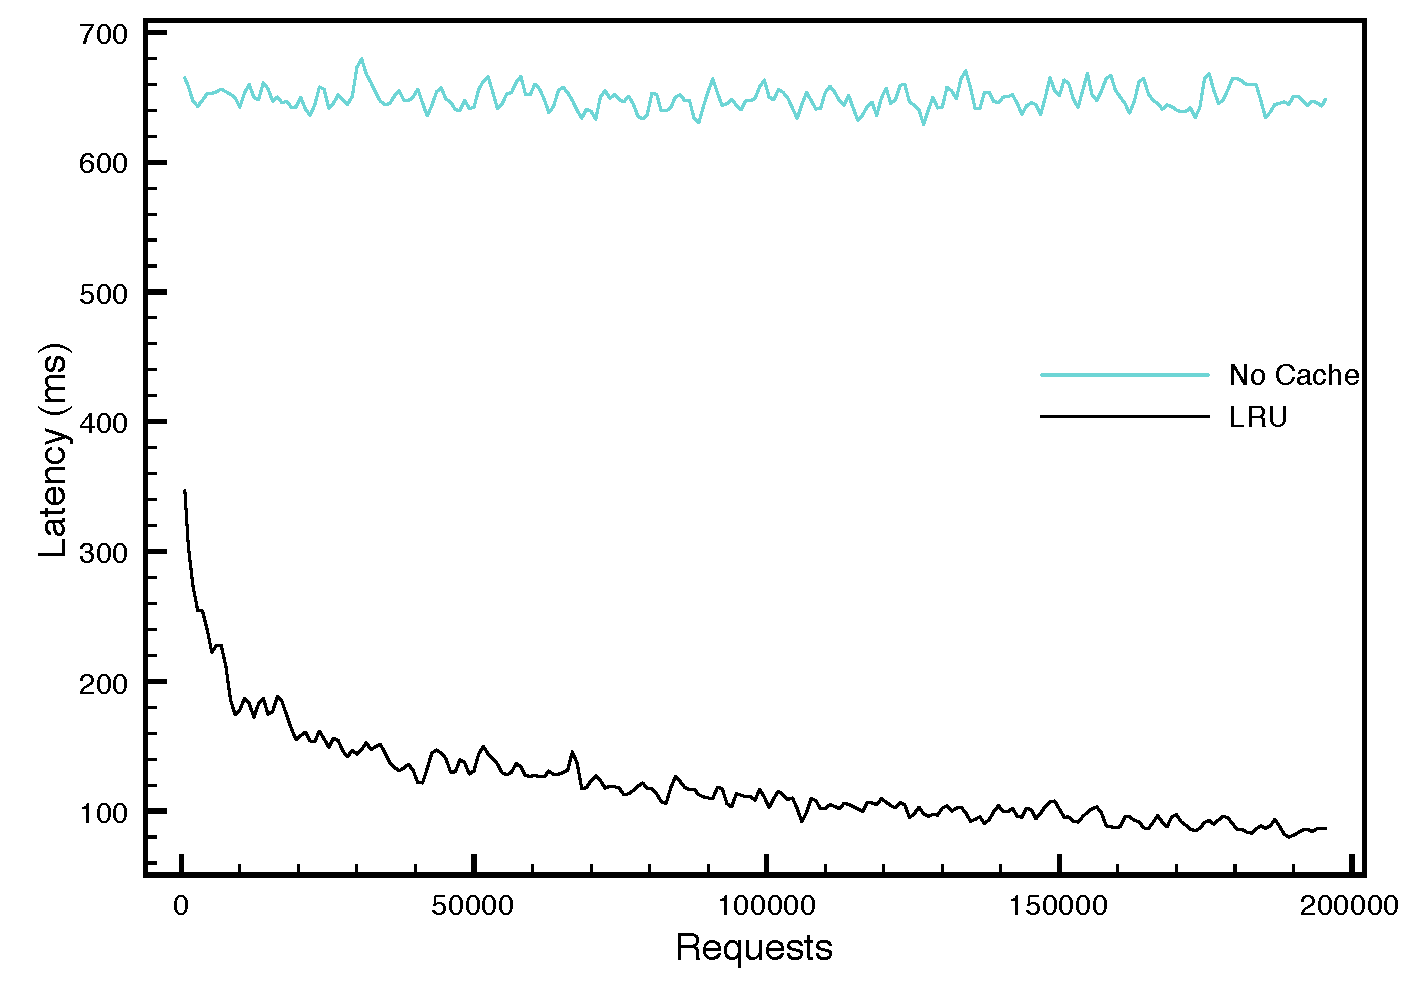
\includegraphics[scale=0.5]{figures/hierarchy-latency-nocache.pdf}
\end{center}
\caption{Query latency for configurations with and without a cache}
\label{fig:hierarchy-latency-nocache}
\end{figure}

Figure~\ref{fig:hierarchy-latency} plots the same LRU-based experimental run as
in Figure~\ref{fig:hierarchy-latency-nocache}, however this time it is
contrasted with a third experimental run that utilized our Cost Aware (CA)
data placement scheme. Although here we do not see such a dramatic speed
increase as the 4x of the last figure, we do see that the Cost Aware solution
does, on average, result in lower query latencies. In the initial 50,000
queries, the gap in time is not quite as pronounced as it is in the remaining
requests. This can be explained as the result of the cached data not having
grown large enough to necessitate eviction from memory or disk, and support the
assertion that the LRU-based solution provides very good average-case
performance. Further, this lends itself to the idea that the Cost Aware scoring
and placement algorithms need time to operate, allowing the scores and data to
settle into place. Based on the trend, had the experiment continued on, LRU was
beginning to level out at a higher average latency than CA.

\begin{figure}
\begin{center}
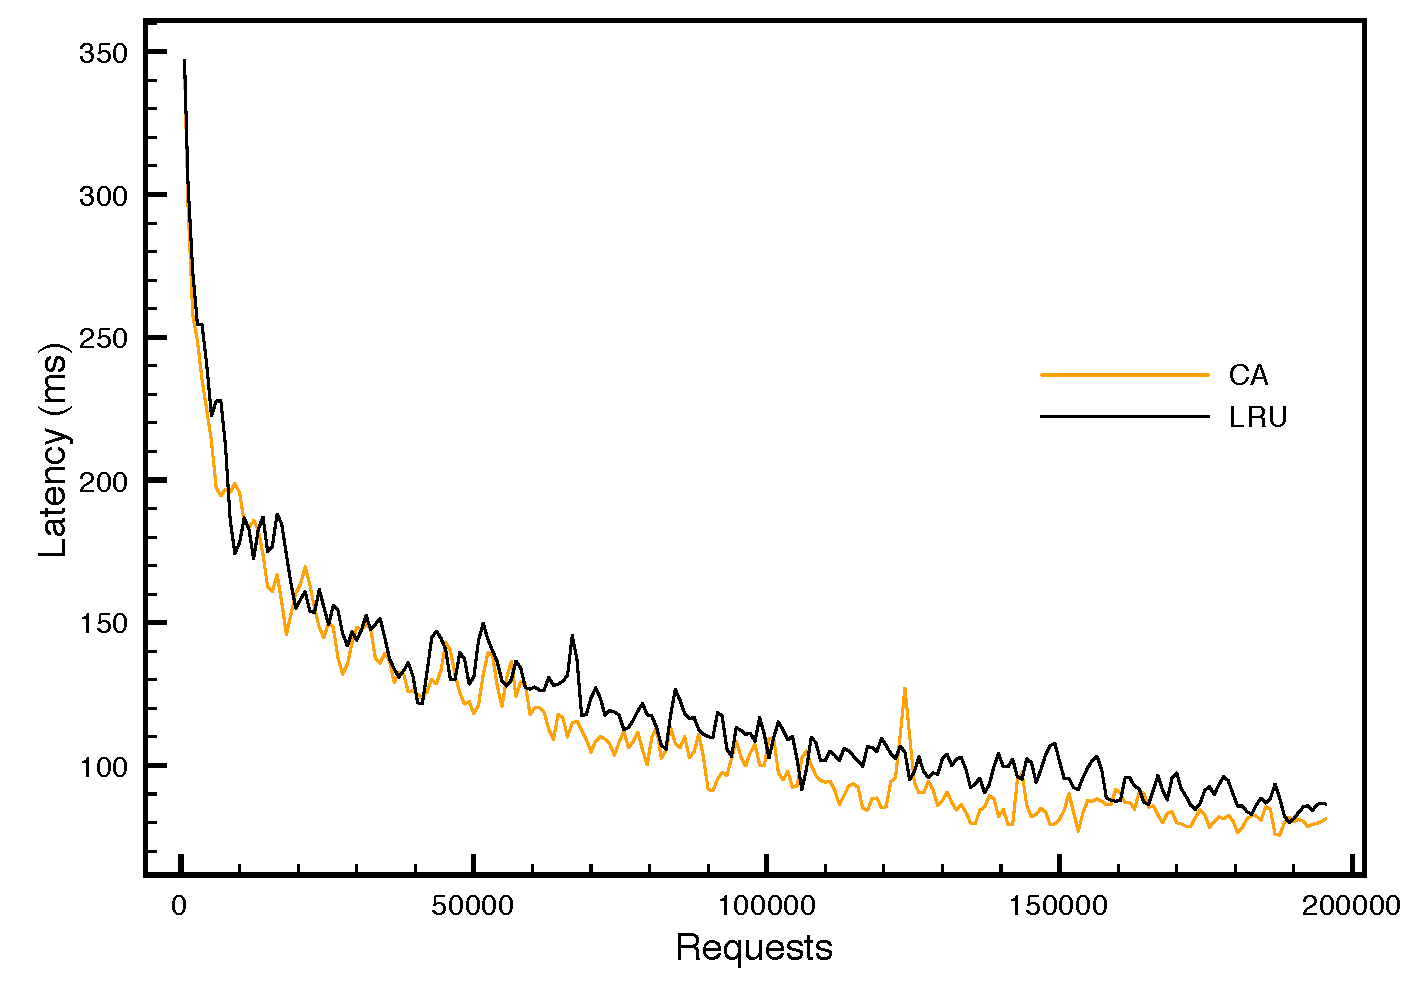
\includegraphics[scale=0.5]{figures/hierarchy-latency.pdf}
\end{center}
\caption{Query latency for CA and LRU data placement schemes}
\label{fig:hierarchy-latency}
\end{figure}

\begin{figure}
  \centering
  \subfigure[LRU Hit Rate]{\
    \label{fig:lru-hitrate}
    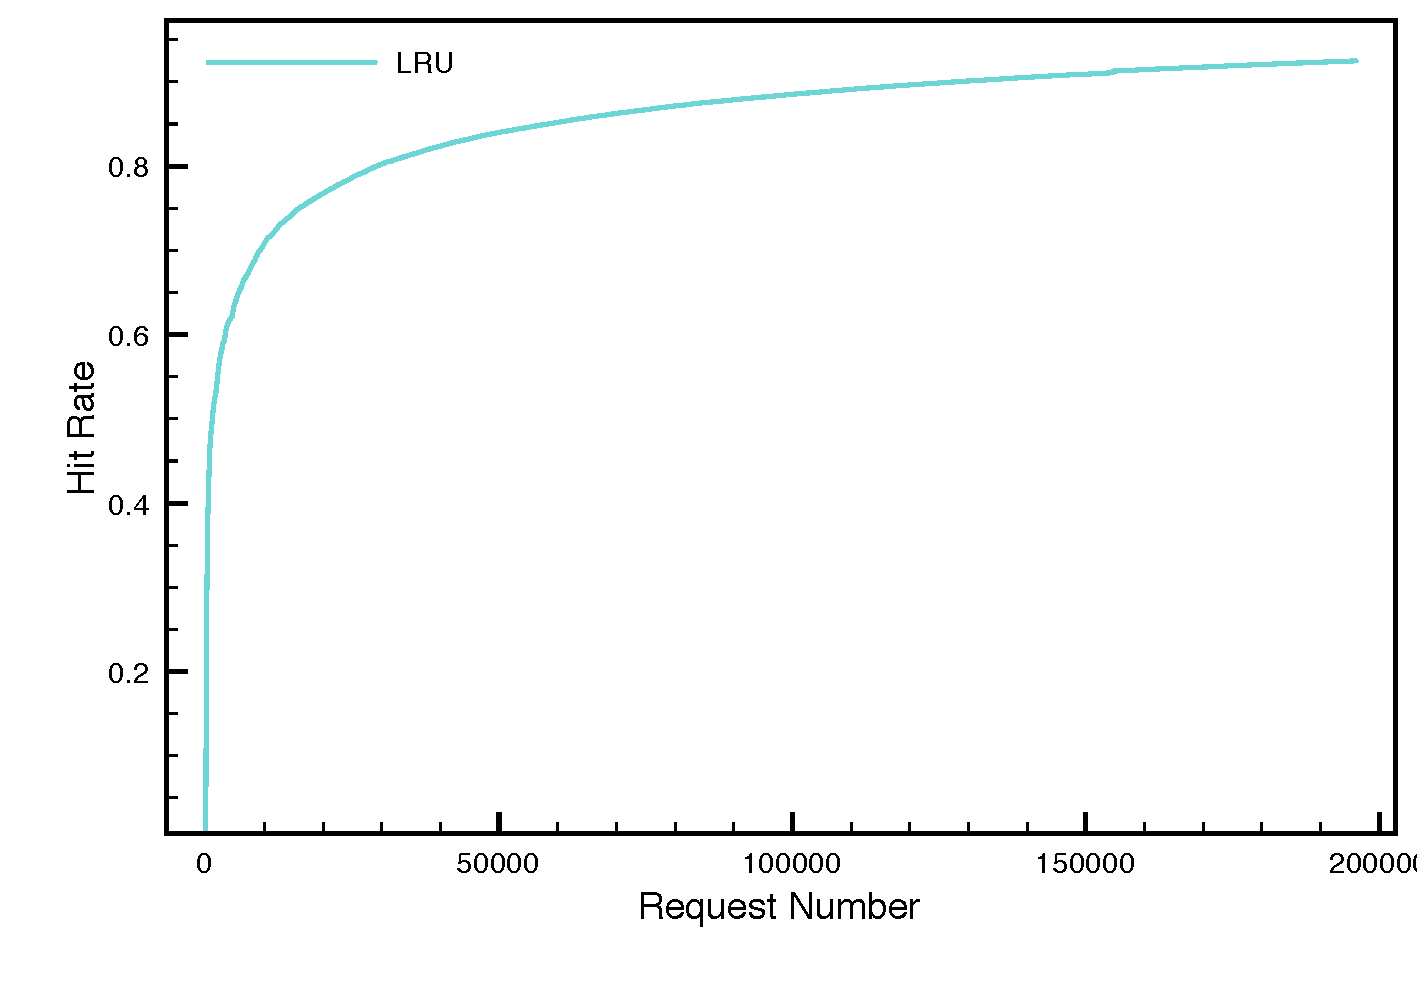
\includegraphics[width=3.3in, trim = 9mm 20mm 0mm 0mm,clip]{figures/lru-hitrate.pdf}
  }
  \subfigure[CA Hit Rate]{\
    \label{fig:ca-hitrate}
    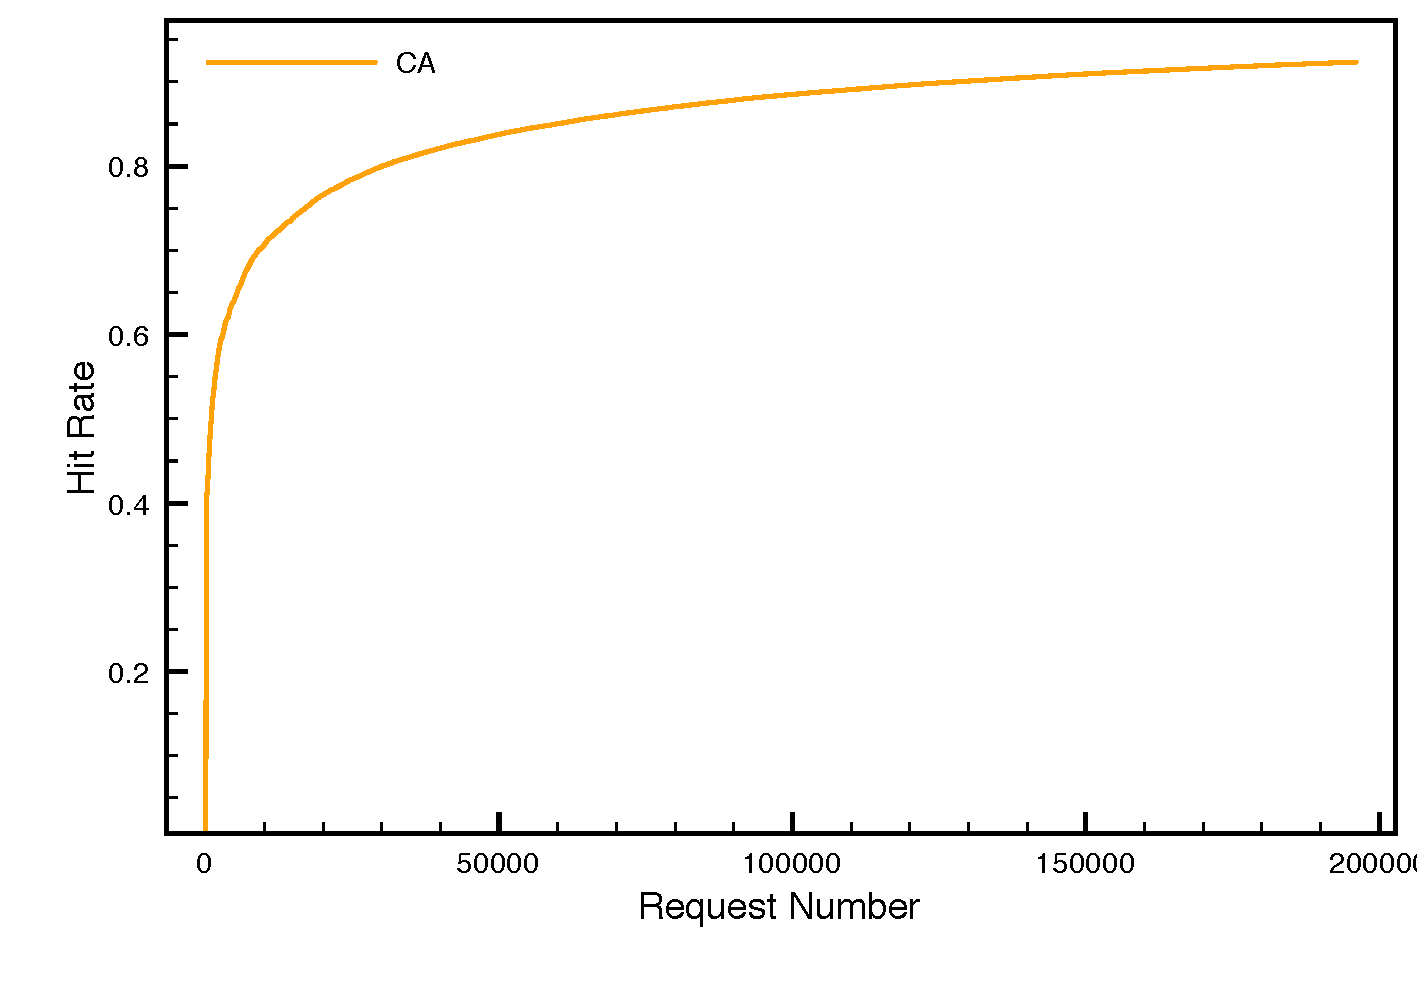
\includegraphics[width=3.3in, trim = 10mm 20mm 0mm 0mm,clip]{figures/ca-hitrate.pdf}
  }\\
	\subfigure[Both Hit Rates]{\
		\label{fig:ca-lru-hitrate}
		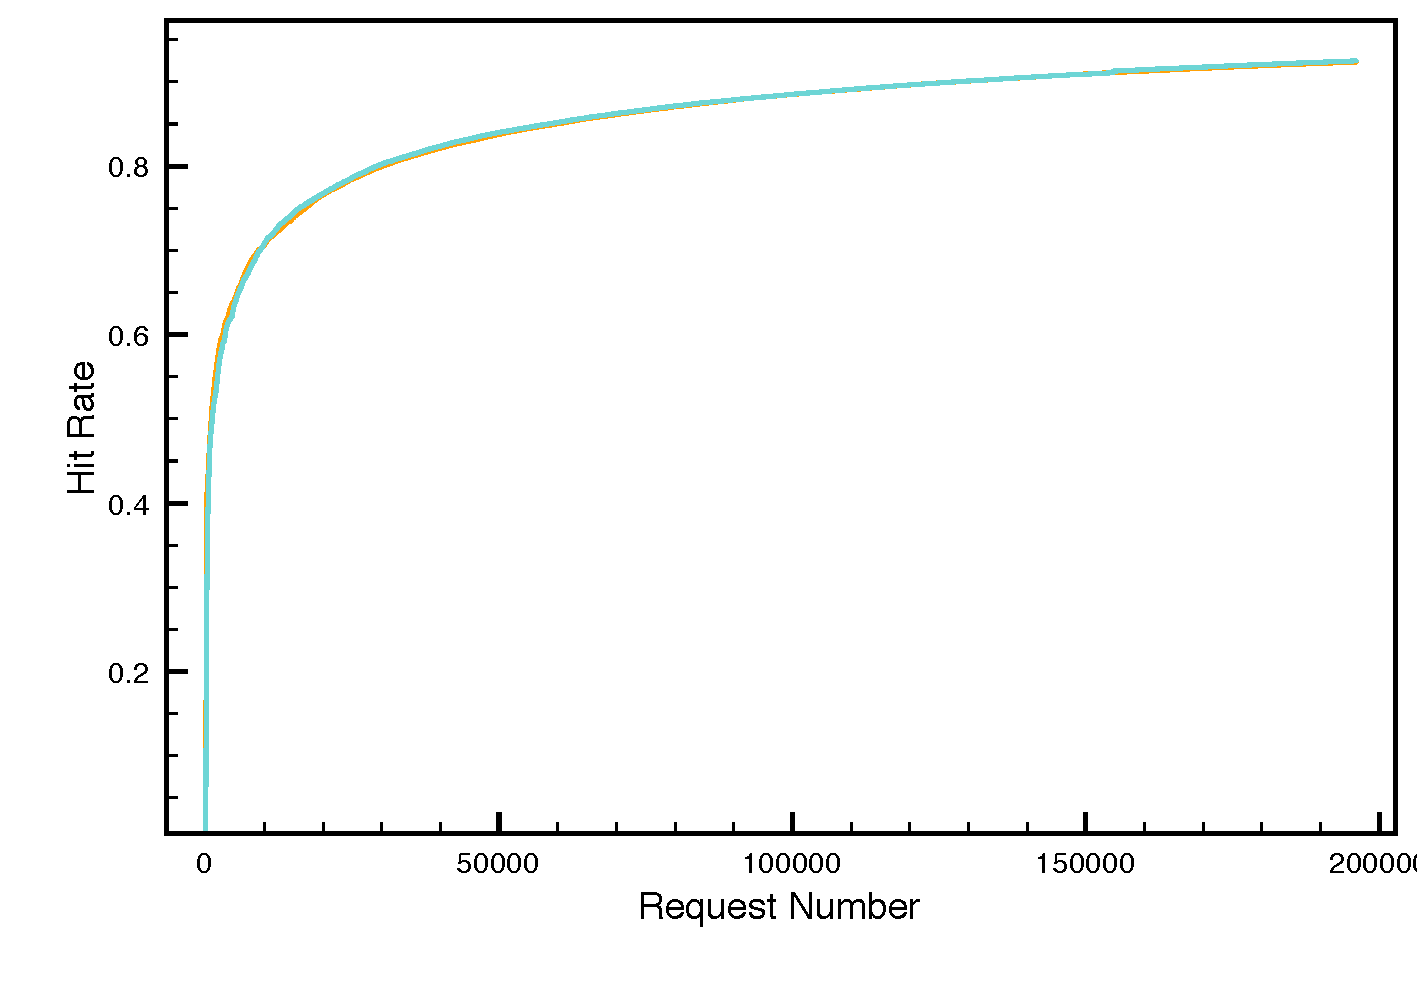
\includegraphics[width=3.3in, trim = 10mm 20mm 0mm 0mm,clip]{figures/hitrates.pdf}
	}
  \caption{Hit Rates by data placement strategy}
  \label{fig:hierarchy-hitrate}
\end{figure}

Figure~\ref{fig:hierarchy-hitrate} presents the cache hit rates for both LRU and
CA (Figure~\ref{fig:lru-hitrate} and~\ref{fig:ca-hitrate} respectively.
Figure~\ref{fig:ca-lru-hitrate} places both lines onto the same graph to
demonstrate that the difference between the two hit rates is minimal at best and
eliminate that as a possible source of the query latency disparity.

\begin{figure}
  \centering
  \subfigure[Hits in memory]{\
    \label{fig:hitloc-mem}
    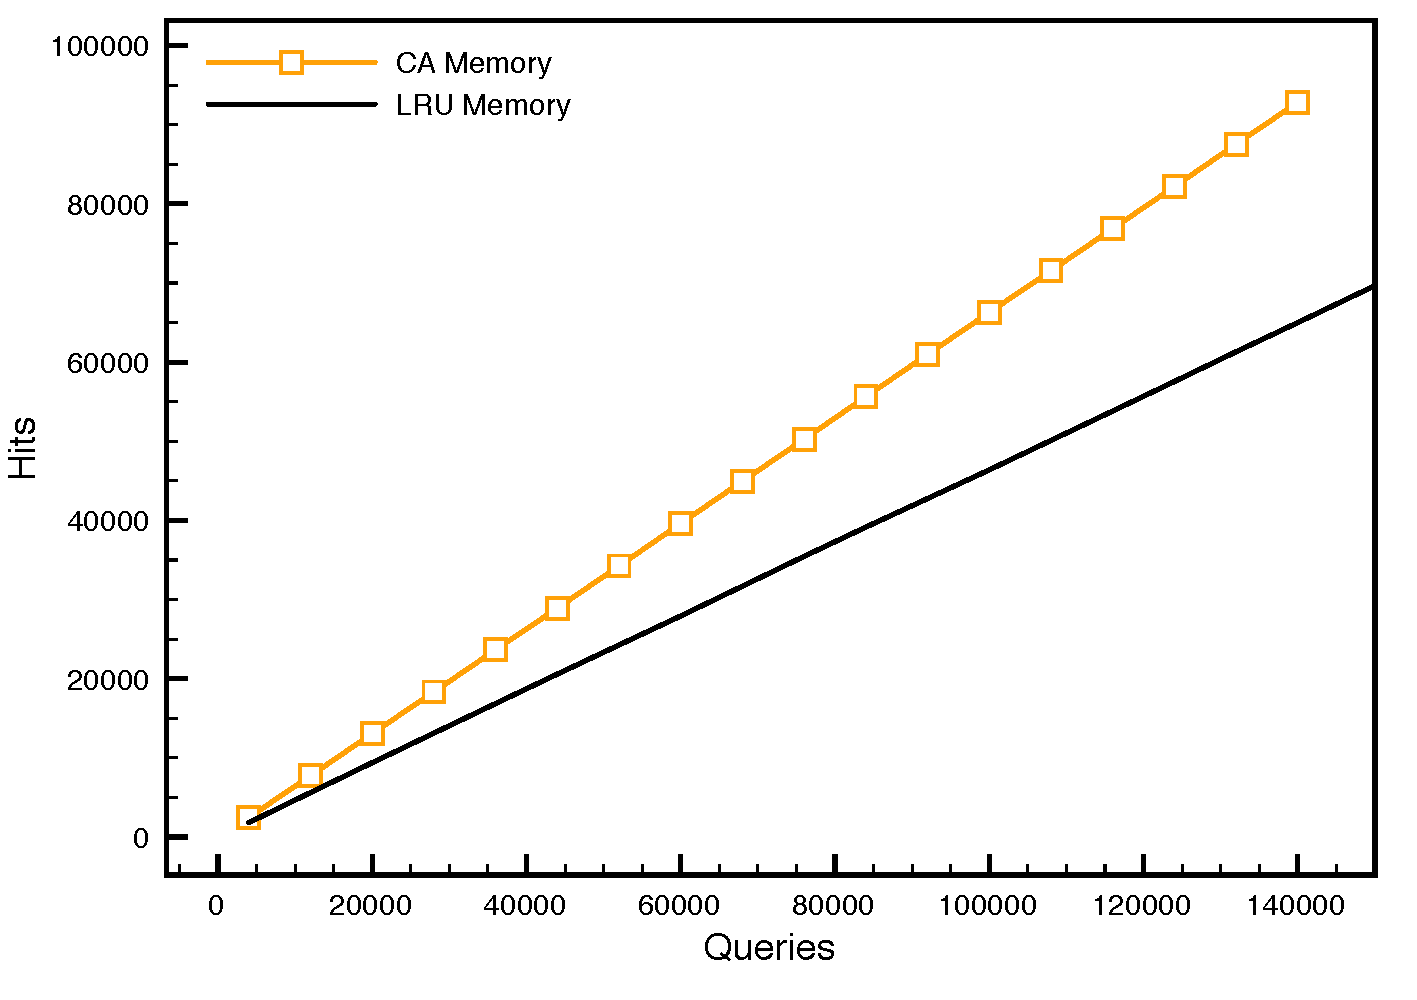
\includegraphics[width=3.3in, trim = 9mm 20mm 0mm 0mm,clip]{figures/hierarchy-hits-mem.pdf}
  }
  \subfigure[Hits on disk]{\
    \label{fig:hitloc-disk}
    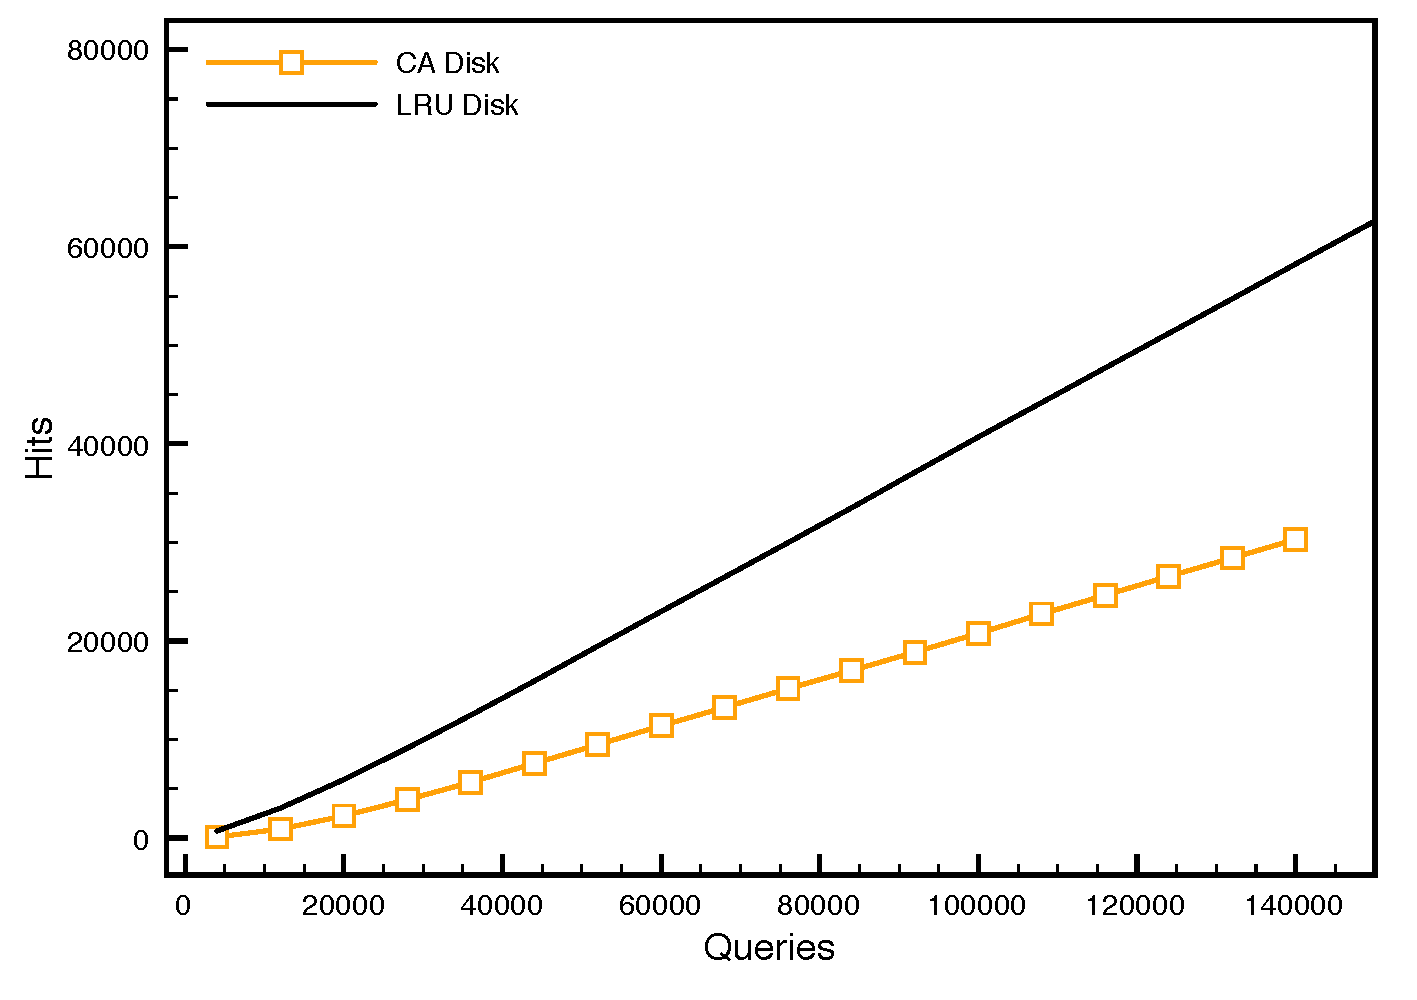
\includegraphics[width=3.3in, trim = 10mm 20mm 0mm 0mm,clip]{figures/hierarchy-hits-disk.pdf}
  }\\
	\subfigure[Hits on cloud]{\
		\label{fig:hitloc-cloud}
		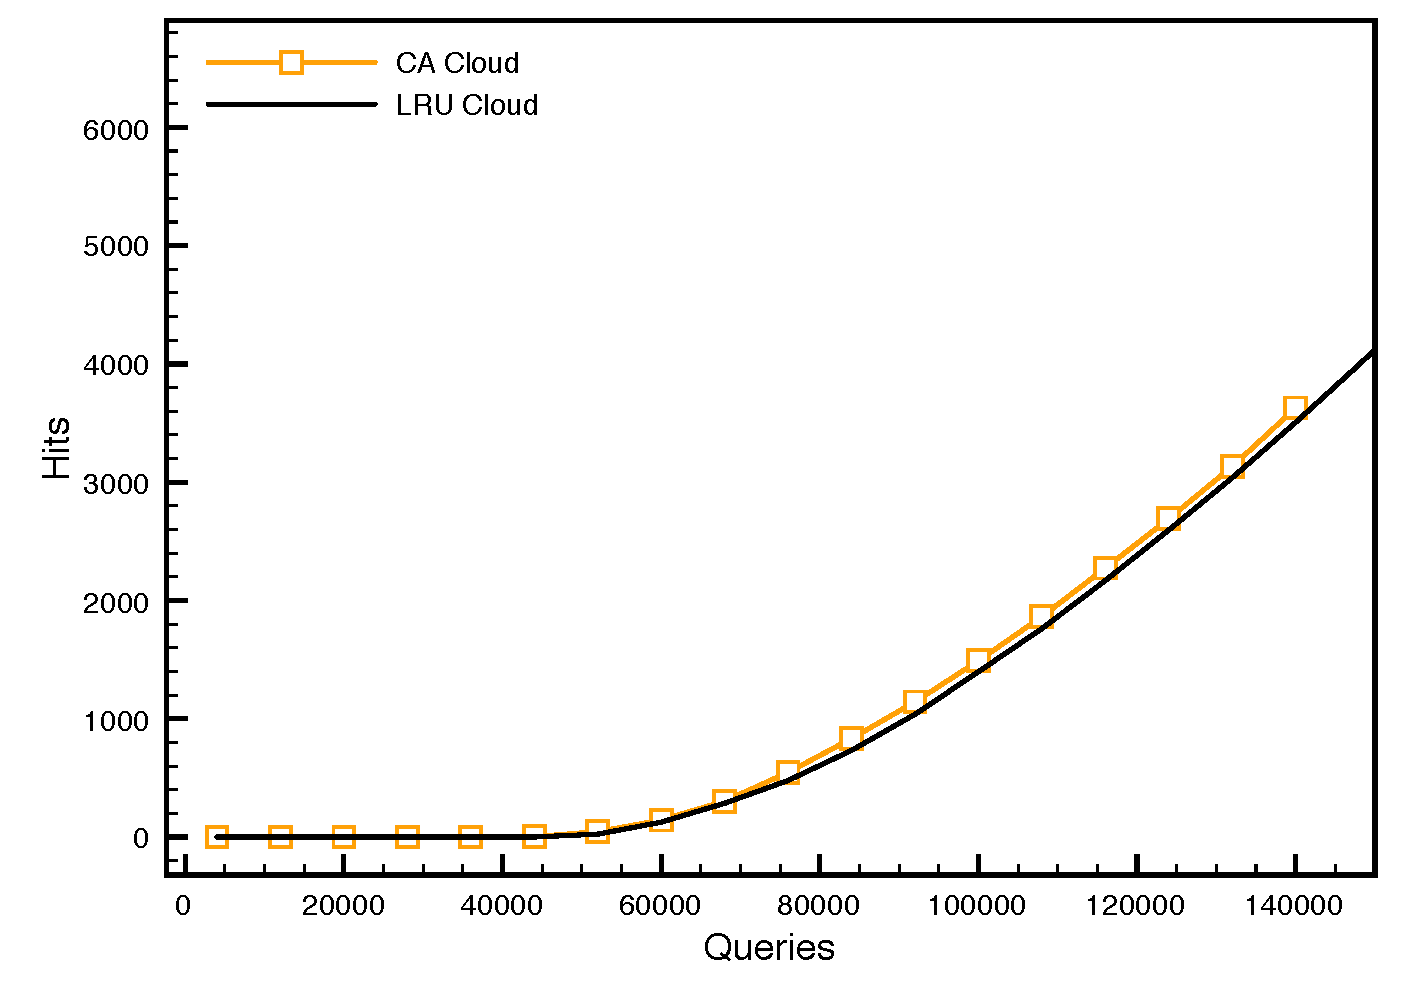
\includegraphics[width=3.3in, trim = 10mm 20mm 0mm 0mm,clip]{figures/hierarchy-hits-cloud.pdf}
	}
  \caption{Hits by hierarchy locations}
  \label{fig:hierarchy-hitloc}
\end{figure}

Finally, we examine the number of hits in each location for each data placement
scheme. Figure~\ref{fig:hitloc-mem} shows that CA results in a greater number
of hits in memory than the LRU-based solution. As a result, in
Figure~\ref{fig:hitloc-disk} we see CA result in fewer hits on disk than LRU\@.
Lastly, Figure~\ref{fig:hitloc-cloud} does not show a significant difference in
the number of hits resulting on the cloud. This is largely due to its
functionality as a last-resort storage medium and the fact that the majority of
the data can be stored within the cache node itself.

% section results_storage (end)
